\section{Solução da calibração}
% TODO Gabriel e Elael: solução detalhada e final da calibração com simulações.

\subsection{Calibração da pá}

A dinâmica do processo de calibração não exige que o algoritmo seja capaz de
identificar qual pá está sendo calibrada, uma vez que a pá que deve ter sua
posição determinada, pode ter seu respectivo modelo informado \textit{a priori}.
Essa característica possibilita descartar a necessidade de comparação e busca de
diversos modelos, reduzindo assim a complexidade computacional. Portanto, é
possível armazenar uma representação de diferentes pás e fornecer, 
como entrada do sistema, o modelo correto de acordo com o tipo de turbina que
está sendo inspecionada.

Os desenhos técnicos das pás, não fornecem informações suficientes
sobre o seu perfil hidráulico e, para fins práticos, os modelos serão adquiridos
a partir da inspeção \textit{in situ} de uma turbina em condições de conservação
que não apresente danos e esse procedimento necessita ser realizado apenas uma
vez para cada modelo. Como especificado em \cite{EMMA DETAIL}, %TODO citar emma
% detail.
o sensor a ser adquirido pelo projeto é o Faro Focus X330. Esse dispositivo
consiste em um \texit{laser scanner} e aquisita a distância percorrida pelo
feixe $laser$ emitido pelo sensor até o obstáculo mais próximo. A partir de um
espelho rotativo e um motor acoplado em sua base, o Focus X330 é capaz de
aquisitar pontos em $360^o$ na horizontal e $300^o$ na vertical. O modelo de
cada pá será, então, uma nuvem de pontos representando tridimensionalmente todas
as caracterísiticas necessárias.

A partir da suposição que a pá se encontra dentro do campo de visão do sensor
$laser$, determinar a posição da pá consiste em posicionar a nuvem de pontos do
modelo de forma que ocorra uma sobreposição entre os pontos do modelo e da cena
e ambos conjuntos de pontos tenham as mesmas características, ou seja,
representem o mesmo objeto. A técnica a ser utilizada é denominada
\textit{correspondence grouping}. 


\subsubsection{\textit{Correspondence Grouping}}
 
O método proposto por \cite{Tombari2010a}, se baseia na identificação de
\textit{features} ou características tridimensionais locais para pontos de
interesse e identificar um conjunto de correspondências entre o modelo 3D e o a
cena analisada, no caso da aplicação do projeto EMMA as corresponências entre a
o modelo da pá e a turbina.

Essa estratégia se baseia na detecção de \textit{features} e descritores locais
para calcular um conjunto de correspondências entre o modelo 3D e a cena a ser
inspecionada. Para a identificação das características, é necessário que
pontos de interesse sejam amostrados tanto do modelo quanto da cena e para cada
ponto é associado um descritor que define as características locais de sua
vizinhaça. Dado os conjuntos de descritores do modelo e da cena a ser analisada,
deve-se então determinar as correspondências entre as correspondências entre os
dois conjuntos, utilizando-se, por exemplo, a distância euclidiana entre os seus
descritores como medida limite. Uma vez que o conjunto de correspondências é
identificado, é realizada uma votação para se identificar se essa característica específica se
encontra ou não na cena. Um acumulador é responsável por contabilizar os votos e
um objeto é detectado caso haja um número suficiente de votos para a sua
presença de em uma determinada posição do espaço. É importante ressaltar que
devido à presença de ruído, aŕeas com muita densidade de objetos ou objetos
parcialmente oclusos, é possível a detecção de falsos positivos, que devem ser
posteriormente tratados.

\subsection{Parâmetros de ajuste}

A técnica de \textit{Correspondence Grouping} tem uma série de parâmetros de
ajuste, como: 

\begin{itemize}
  \item \textit{Model/Scene uniform sampling radius} - O processo de
  \textit{uniform sampling} subamostra e uniformiza a nuvem de pontos da cena
  analisada e, também, do modelo de comparação em um número reduzido de pontos
  chave.
  Essa etapa é realizada sobrepondo uma grade 3D de voxels sobre a nuvem de
  pontos e calculando o centróide de cada voxel.  O raio (\textit{uniform
  sampling radius}) ou tamanho da folha dessa grade dita, então, quanto a
  resolução da nuvem de pontos será reduzida.
  \item \textit{Reference frame radius} - Para se obter descritores invariantes
  a pose dos objetos analisados, é implementada a utilização de um sistema de
  coordenada local associado a cada ponto chave da nuvem de pontos. Essa é etapa
  é regulada pela distância máxima dos pontos utlizados para se estimar os
  eixos $x$ e $y$ do sistema de coordenada local de cada ponto
  (\textit{Reference frame radius}).
  \item \textit{Descriptor radius} - Raio da esfera usada para determinar a
  vizinhaça de cada ponto utilizada na estimação de \textit{features}.
  \item \textit{Cluster size} - Define o tamanho da célula no espaço de
  Hough, utilizado para votação. %TODO VERIFICAR TRADUÇÂO
  \item \textit{Clustering threshold} - Define o número mínimo de votos
  necessário para indicara presença de uma instância do modelo na nuvem de
  pontos da cena de entrada. \end{itemize}

Esses parâmetros devem ser ajustados para cada tipo de aplicação em que se
deseja reconhecer objetos e também é dependente das características presentes em
cada modelo, como sua resolução e densidade por exemplo. Devido a essa
caracterísitica, é importante que seja possível replicar as características que
serão encontradas no cenário real de utilização do algoritmo de calibração. 

\section{Simulação de nuvem de Pontos}

A utilização de dados sintéticos para a implementação e ajuste de algoritmos é
uma prática aplicada amplamente e possibilita o gradual aumento na complexidade
dos dados introduzidos no algoritmo e descoberta e entendimento das nuances
específicas do problema.

\subsection{Dados genéricos}

Para um primeiro contato com o funcionamento do método \textit{Correspondence
Grouping} foi utilizado dados genéricos disponíveis na literatura e foi
introduzido artificialmente o modelo da pá gerado pelo sensor Faro Focus X330,
durante a viagem de campo à Usina Hidrelética de Jirau para o teste de
viabilidade técnica desse sensor. 

A figura \ref{fig::modelo_pa_faro} ilustra o modelo da pá em nuvem de pontos,
esse modelo é uma representação de $360^o$ da superfície da pá e foi aquisitado em
campo, sendo assim representa a real leitura final do sensor na aplicação do
algoritmo de calibração.

\begin{figure}[h!]
	\centering
	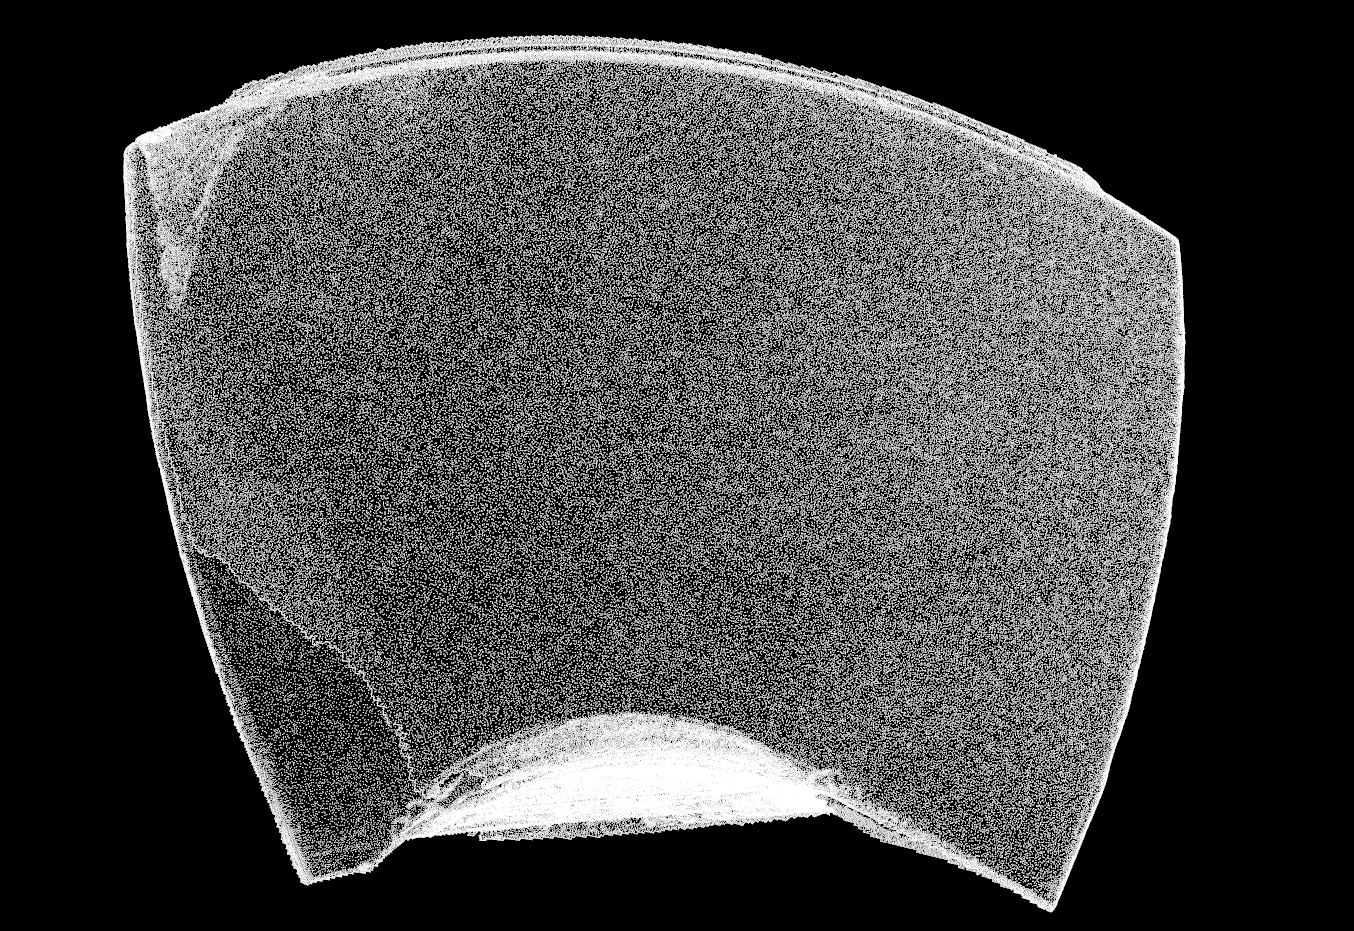
\includegraphics[width=0.6\columnwidth]{figs/calibracao/modelo_pa_faro}
	\caption{Nuvem de pontos da pá aquisitada pelo sensor Faro Focus X330.}
    \label{fig::modelo_pa_faro}
\end{figure}

A identificação da objeto na cena e a estimação da sua posição foi testada em
uma cena de um escritório, como pode ser visualizado na figura
\ref{fig::pa_cena_gen}. Pode-se verificar que mesmo com uma diferença de
densidade de pontos presente em cada parte da nuvem de pontos resultante (cena
e modelo da pá), foi possível realizar a correta localização do modelo. O
ajusteo dos paramêtros de subamostragem dos modelos e da cena necessitaram de
maior atenção nesse cenário. Vale ressaltar que o algoritmo identificou
corretamente uma cópia exata do modelo que foi introduzido na cena, não há
presença de ruídos ou oclusôes.

\begin{figure}[h!]
	\centering
	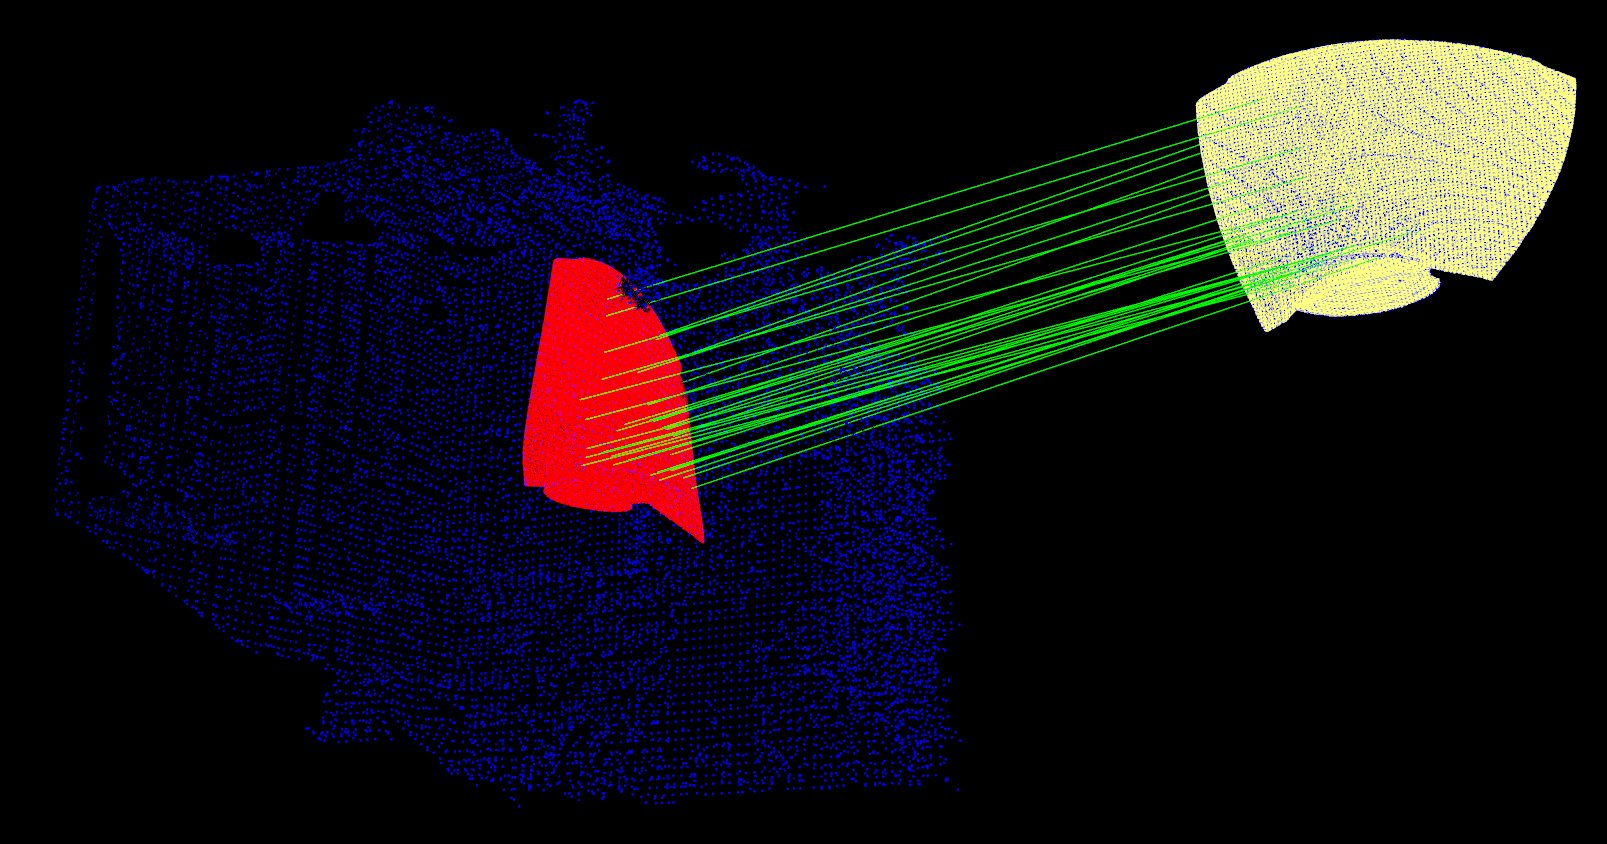
\includegraphics[width=0.6\columnwidth]{figs/calibracao/pa_cena_gen}
	\caption{Exemplo de localização do modelo da pá em uma cena genérica.}
    \label{fig::pa_cena_gen}
\end{figure}

\subsection{Blensor}

Uma alternativa para a criação de dados, nos quais existe a presença de oclusão,
é a simulação do sensor utilizado e a projeção da sombra de um objeto que se
encontra entre o sensor e o alvo original. Para a simulação desses cenários, foi
utilizado a \textit{toolbox Blensor}\footnotemark
\footnotetext{http://www.blensor.org} baseada no \textit{software} de criação 3D
\textit{Blender}\footnotemark \footnotetext{http://www.blender.org}, o qual
permite a simulação da nuvem de pontos resultante de um sensor em um ambiente
tridimensional. Os objetos inseridos na cena são sólidos 3D, que podem ser
desenhados utilizando-se as ferramentas do próprio programa ou importados de
outros programa que utilização formatos suportados, como o Solidworks por
exemplo. A Figura \ref{fig::blensor_screen} ilustra a utilização do software,
assim como o modelo 3D da turbina importado. A simulação leva em consideração a
distância percorrida pelo pulso emitido, a intensidade luminosa retornada ao
sensor e o tempo decorrido durante o sensoriamento \cite{Gschwandtner2011}, o
que fornece uma melhor aproximação da resposta do sensor para um ambiente
simulado do que simplesmente a utilização de uma técnica de \textit{raycast} pura.

\begin{figure}[h!]
	\centering
	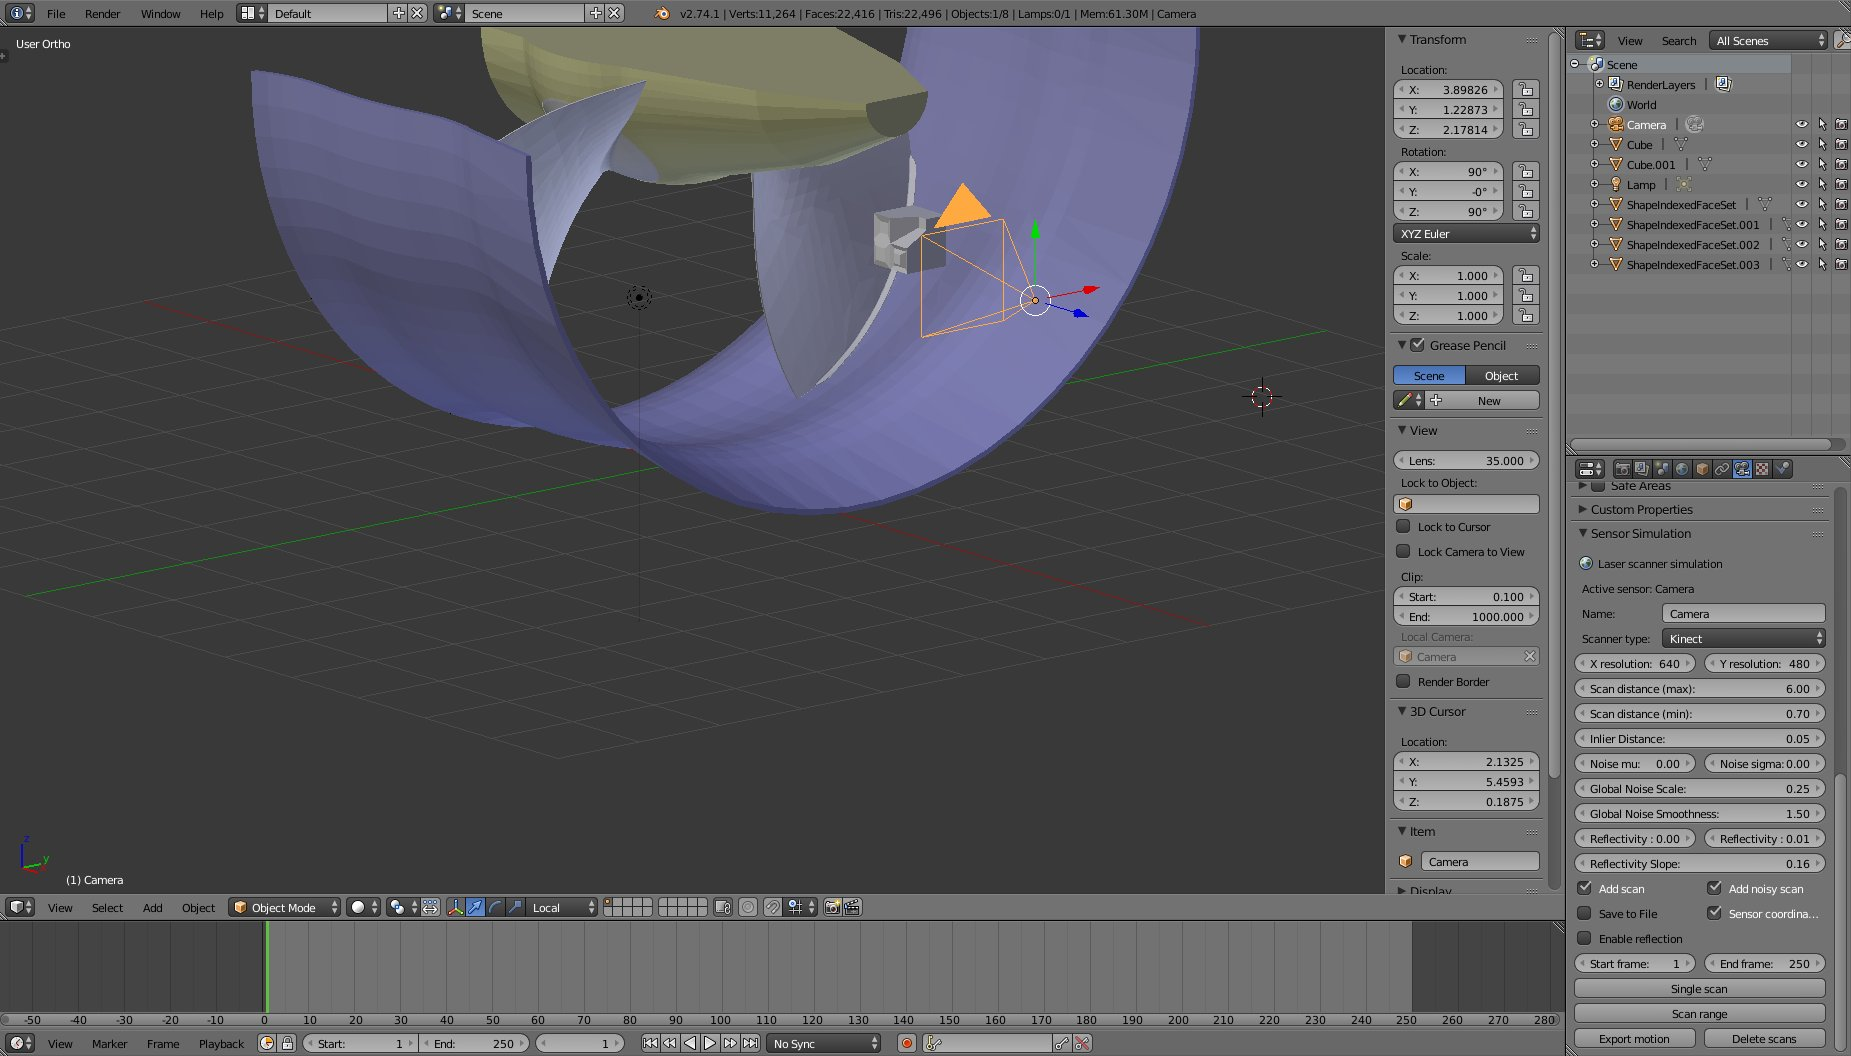
\includegraphics[width=0.9\columnwidth]{figs/calibracao/blensor_screen}
	\caption{Visualização do \textit{Blensor} com o modelo 3D da turbina
	importado.}
    \label{fig::blensor_screen}
\end{figure}

Dentro do ambiente de simulação, é possível a sintetização de dados provenientes
de diversos tipos de sensores laser, como um laserscanner 2D, Velodyne e
sensores do tipo kinect. Os parâmetros de configuração dos sensores também estão
disponíveis para ajuste, assim como o nível de ruído. Sensores que não estão
nativamente disponíveis também podem ser introduzidos e, assim, o sensor Faro
Focus X330 pode ser simulado, como ilustrado na Figura \ref{fig::blensor_faro}.

\begin{figure}[H]
	\centering
	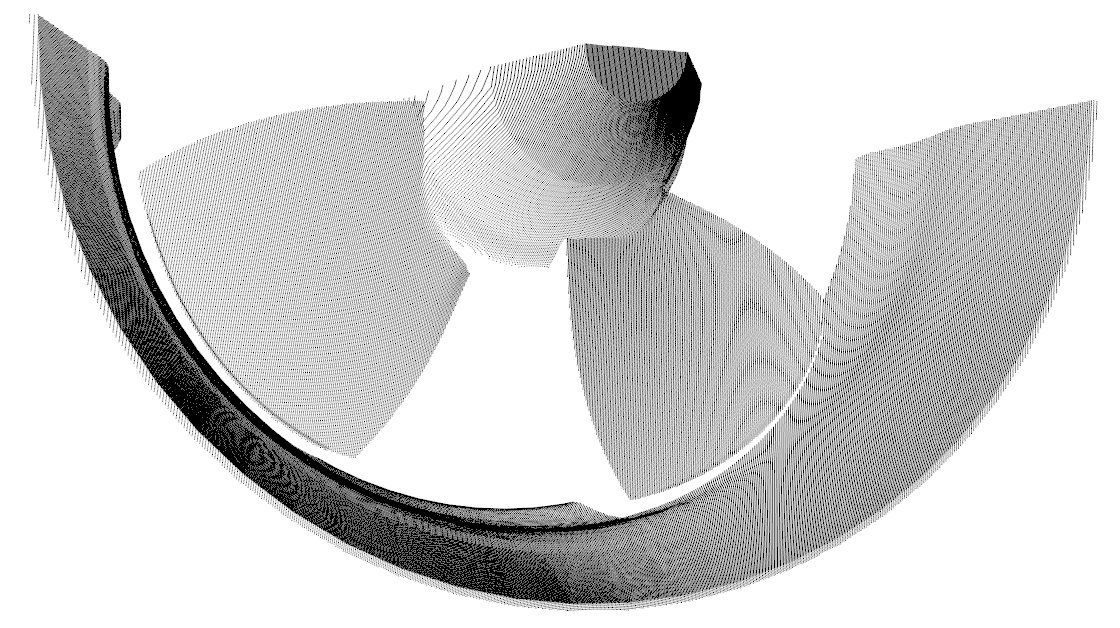
\includegraphics[width=0.9\columnwidth]{figs/calibracao/blensor_faro}
	\caption{Resposta simulada do sensor Faro Focus X330.}
    \label{fig::blensor_faro}
\end{figure}	


Com o ambiente de simulação configurado, é possível explorar diversos níveis de
oclusão, assim como posicionamentos do sensor. O modelo 3D do manipulador
Motoman MH12 utilizado também foi importado e foi utilizado como obstáculo para
a identificação da pá na nuvem de pontos sintética. A Figura \ref{fig::sim_mh12}
ilustra a pá sendo corretamente identificada com a presença do manipulador entre
o sensor e a pá criando uma região de sombra.

\begin{figure}[H]
	\centering
	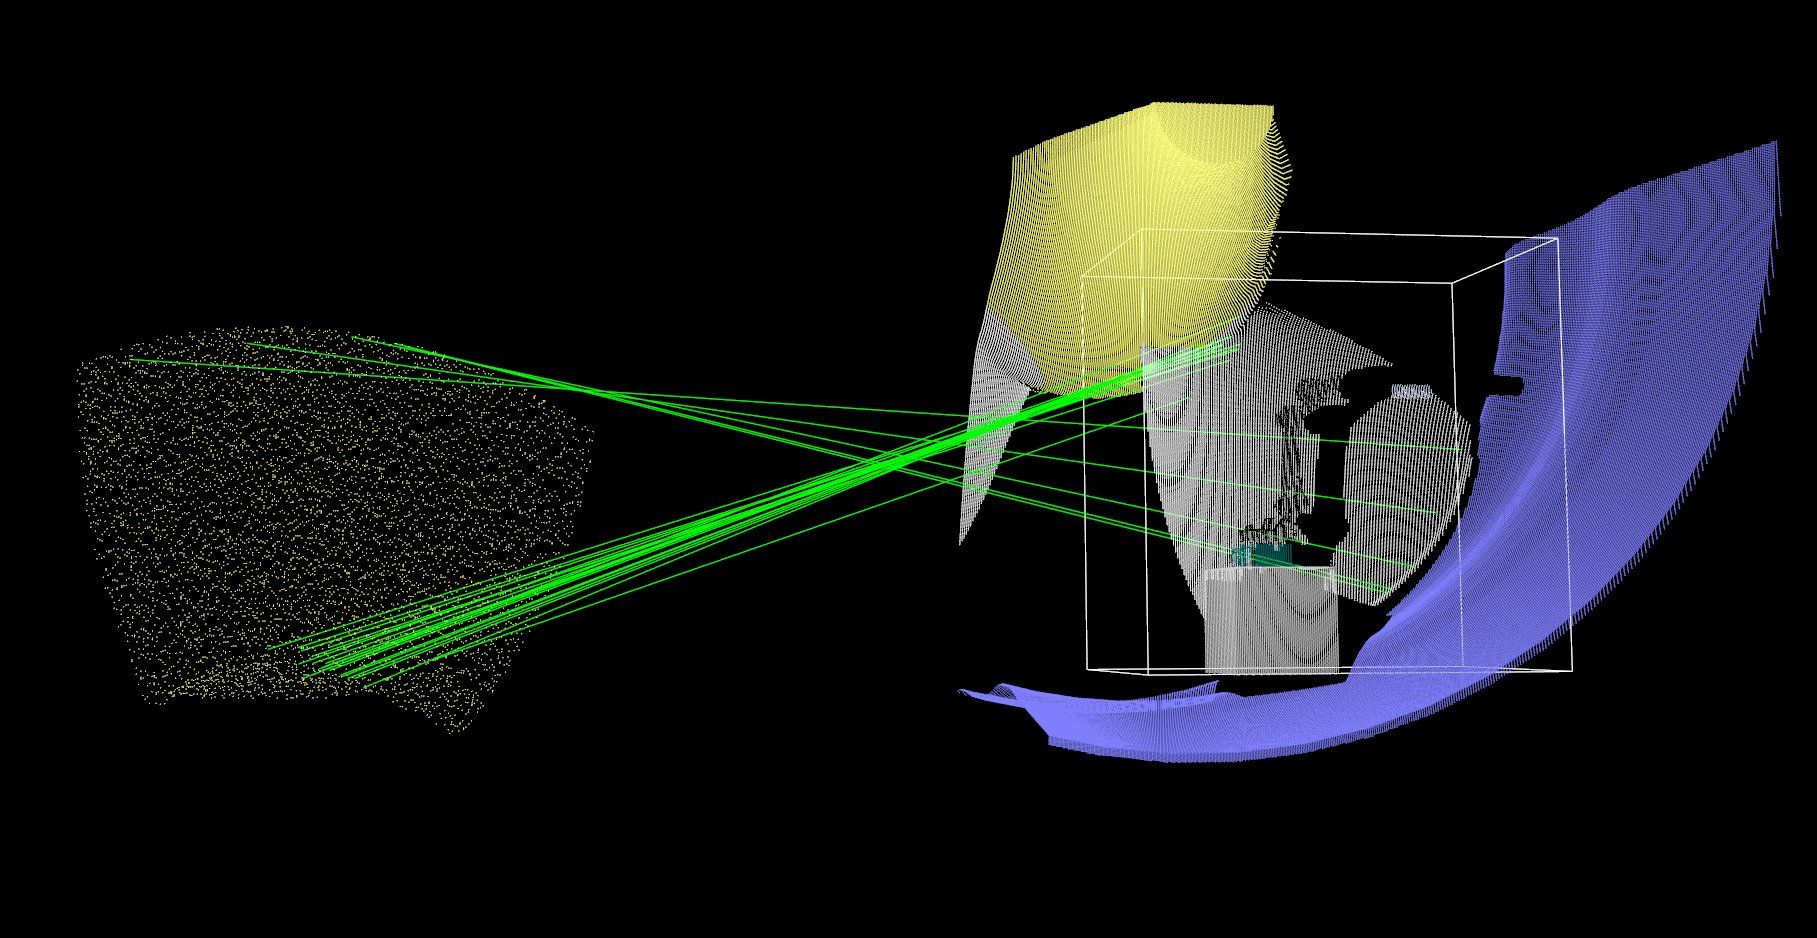
\includegraphics[width=0.9\columnwidth]{figs/calibracao/sim_mh12}
	\caption{Resposta simulada do sensor Faro Focus X330.}
    \label{fig::sim_mh12}
\end{figure}	
